\subsection{Exploring space}
\label{sec:impbehavior}

%\begin{figure*}[htbp]
%\centerline{
%\includegraphics[width=2.8in, angle=270 ]{./figures/GrabSeq.eps}
%} \caption[An example of the Grasping Behavior]{Grasping behavior:
%an example. Sequence of the robot grasping a porcelain cup. Frame
%1: the cup is presented to the robot. Frame 2: the robot reaches
%for the cup. Frames 3 to 6: the robot explores the space and uses
%tactile feedback to find the object and adjust the position of the
%hand. Frames 7 and 8: the robot grasps and lifts the cup.}
%\label{fig:sequence}
%\end{figure*}

We assume that the robot's arm starts at a position above the
table. The hand has its thumb up and the index and middle fingers
extended. When a person waves an object(motion
detection\cite{kemp-thesis}) in front of the robot, the robot
moves its hand towards the object using the 2D information of the
camera and the kinematics information from the head and the arm.
The third dimension is given by the height of the table that the
arm originally detected.

After the reaching motion and if not contact has been detected, an
exploration around this position is performed. The hand is moved
to the side and to the front parallel to the table. These
directions are computed using the kinematics of the arm.

If contact with the hand is detected, the exploration is stopped
and the thumb is rotated to oppose the index finger. Then, the
hand is repositioned depending on where the contact occurred.(*)
If only the index finger is in contact with the object, the hand
is moved down until contact with the table.
%
If there is not contact with the palm, the arm will be moved in
the direction of the forearm until contact occurs.
%
Once in contact with the palm, the fingers will be closed ...
%
If the operation fails a the arm will be returned to the initial
position.


\section{Evaluations}
\label{sec:results}

\begin{table*}[htb]
  \caption{Objects.} \label{tab:objects} \centering
  \begin{tabular}{|c|l|c|c|c|l|}
    \hline
    &Description& Weight(Kg)&No.Trials&No.Failures&Contains \\
    %&Object& W(Kg)&Trials&Fail&Contains \\
    \hline
    1&Plastic bottle        & 0.265 & 22& 0 & Vitamins\\
    2&Porcelain cup & 0.255 & 24& 1 & Nothing\\
    3&Plastic cup (Starbucks)      & 0.220 & 24& 4 & Bolts \\
    4&Rectangular box (Nesquick)        & 0.240 & 24& 2 & Nesquick powder\\

    \hline
  \end{tabular}
\end{table*}

\begin{figure*}[tbp]
\centerline{
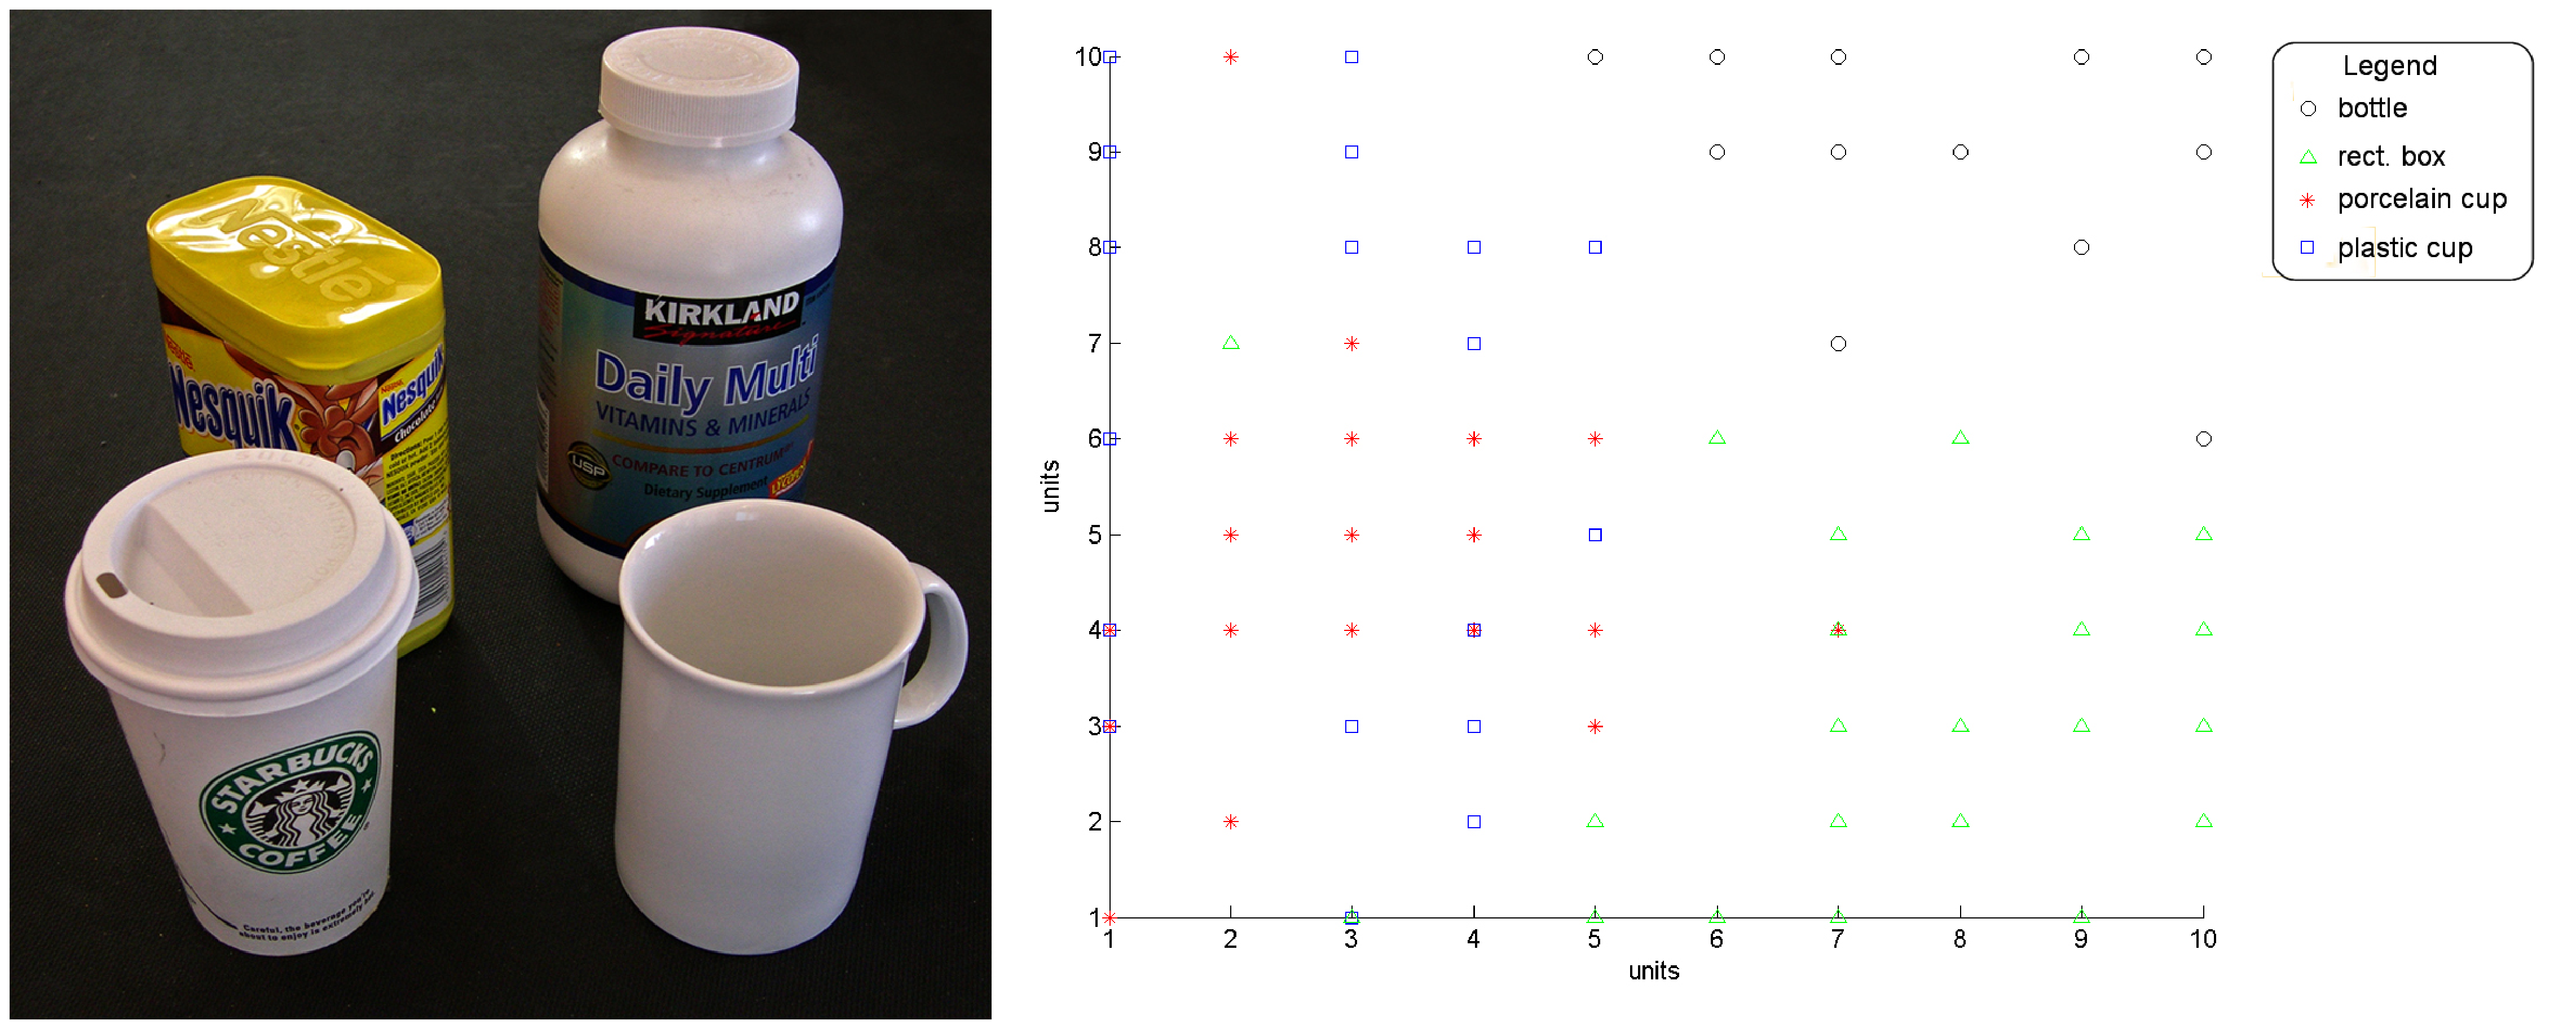
\includegraphics[width=6.0in]{./figures/objects-clusters2.eps}
}\caption[Objects grabbed and clustering]{Left: the set of objects
used in the experiments: a plastic bottle, a porcelain cup, a
plastic cup and a rectangular plastic box. Some objects were
partially filled to increase the weight (all objects weighed about
220-250g). Right: result of the clustering. Black circles, green
triangles, red stars and blue squares represent respectively the
bottle, the rectangular box and the porcelain and the plastic
cups. The two cups are not clearly separated because they have
similar shape in the area where they were grasped.}
\label{fig:Objects}
\end{figure*}

%% \begin{figure}[tbp]
%% \centerline{
%% 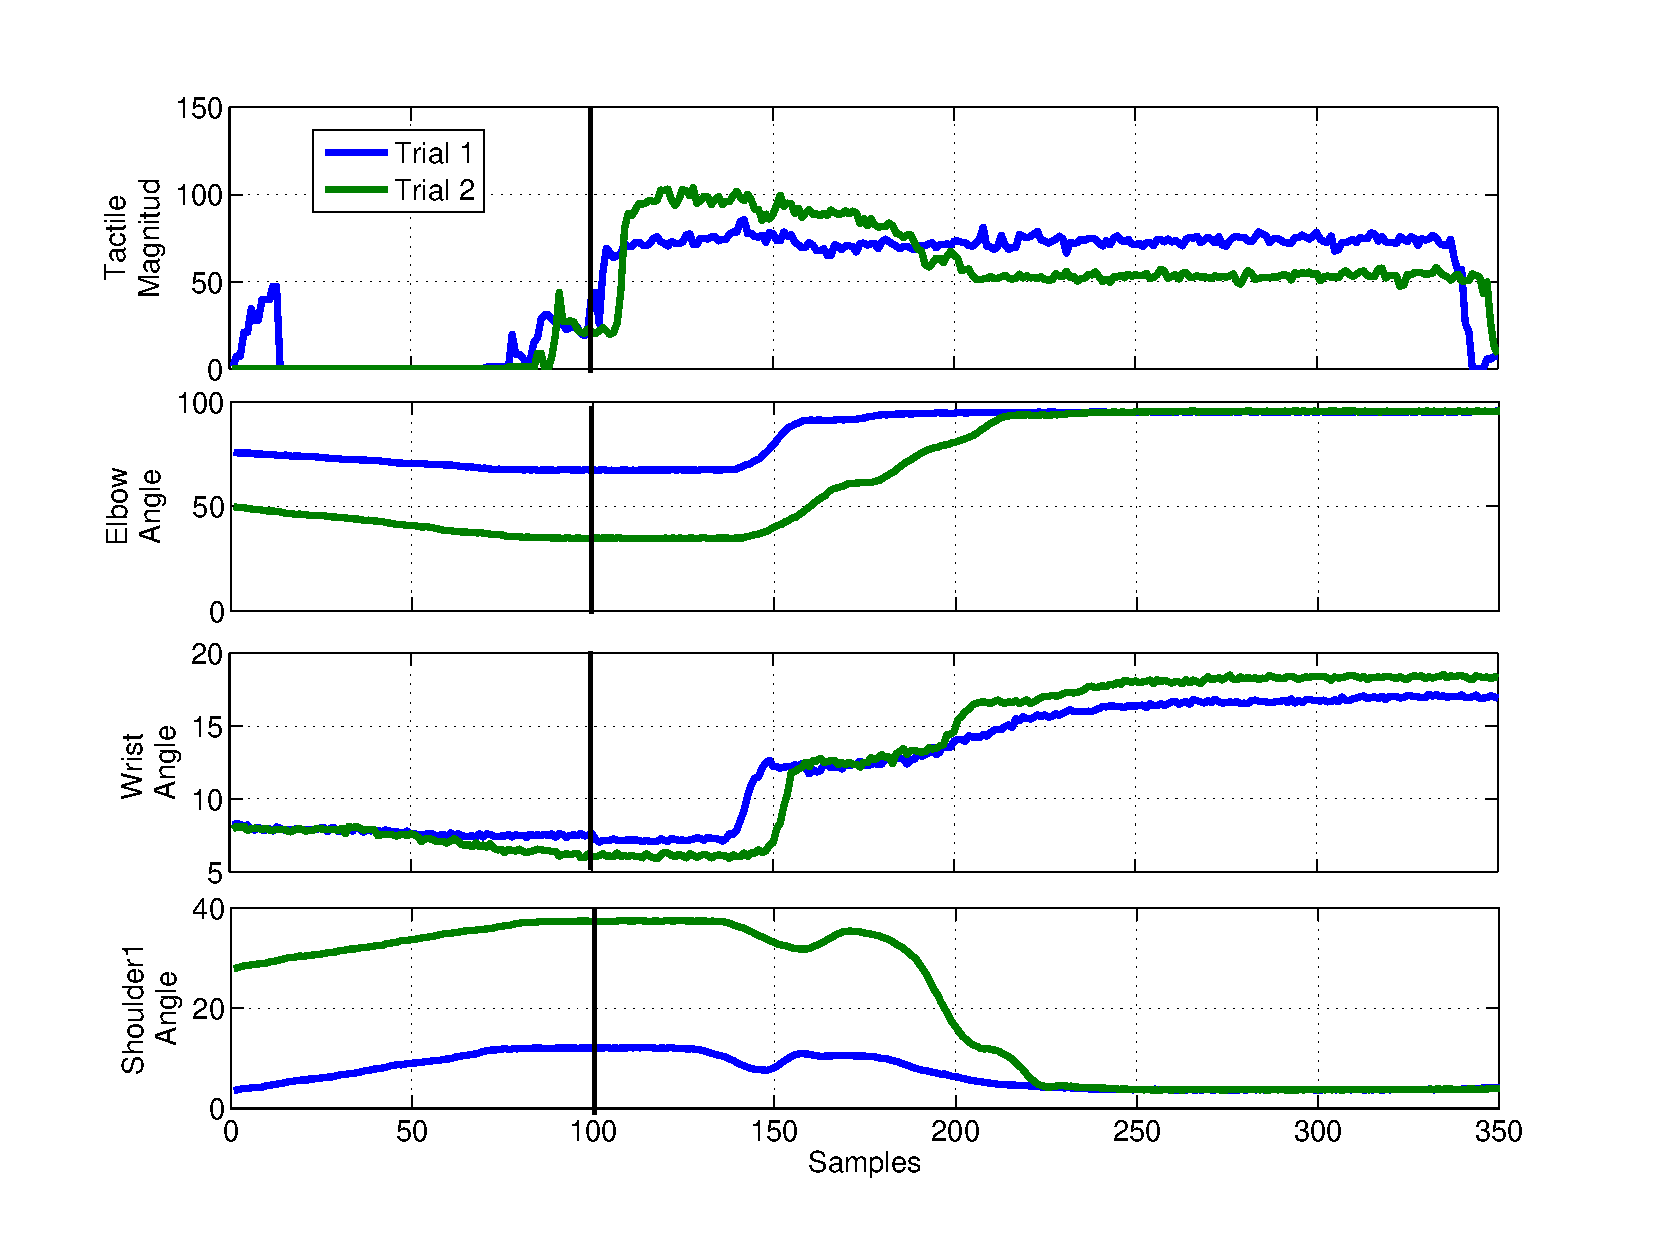
\includegraphics[width=3.5in]{./figures/GraspingData1.eps}
%% }\caption{The figure presents the trajectories followed by two
%% different grasping sequences of a same object. We can observe that
%% the tactile sensor response capture the variation in the different
%% trajectories. The magnitude of the tactile vector is the vectorial
%% summation of the forces present in each tactile sensor considering
%% the current geometry of the hand.} \label{fig:AnglesPlot}
%% \end{figure}

%% \begin{figure}[tbp]
%% \centerline{
%% 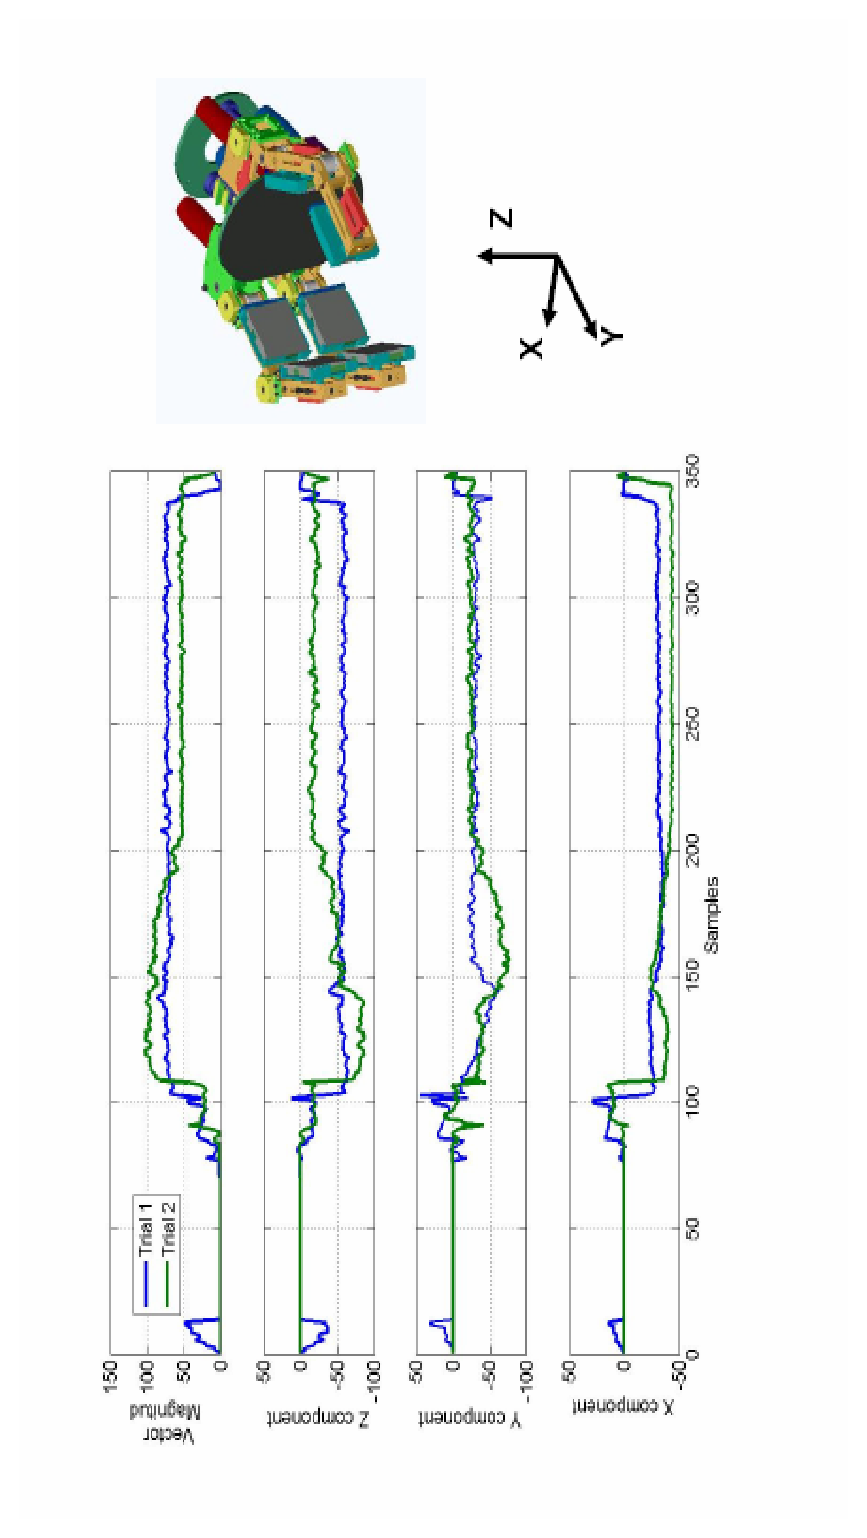
\includegraphics[height=3.2in, angle=270]{./figures/TactileComp.eps}
%% }\caption{The magnitude of the tactile vector is the vectorial
%% summation of the forces present in each tactile sensor considering
%% the current geometry of the hand.} \label{fig:TactileComp}
%% \end{figure}

The grasping described in Section~\ref{sec:controlling} was
evaluated by presenting different objects to the robot and by
counting the number of successful grasps. We chose objects of
different size and shape: a plastic bottle, a plastic rectangular
box, a porcelain cup and a plastic cup (see
figure~\ref{fig:Objects}). Some of the objects were partially
filled, so that the weight was roughly uniform among all objects
(about 220-250 grams, see Table~\ref{tab:objects}). The robot had
no prior knowledge about these objects.

Each object was presented to the robot more than 20 times and
randomly placed on the table. Overall the number of grasping
trials was 94, of which only 7 were not successful. In some of
these trials, the robot managed to grasp the object, but was not
able to hold it because the grip did not produce enough friction.
In a few cases the tactile sensors failed to detect the object and
the exploration was aborted before the object was actually grasped
(more details are reported in Table~\ref{tab:objects}).

As a further validation, we clustered the haptic information
originated from the grasping. We collected the hand feedback at
the moment the robot lifted the object; the idea is that given the
intrinsic compliance of the hand, its configuration and the force
exerted by each joint depend on the shape of the object being
grasped. The hand feedback was clustered by means of a Self
Organizing Map (SOM). The results show that the bottle, the
rectangular box and the cups form three clusters. Unfortunately
the clusters formed by the two cups are not clearly
distinguishable. This is probably due to the fact that the hand
grasped the objects from the top, and that in that part the two
objects are quite alike (both are circular with similar diameter).
In these cases the limited number of fingers (three) made it hard
to distinguish between the cylindrical and conic shape of the
cups. Together the results prove that the \emph{grasping} behavior
of the robot is reliable. The high number of successful trials
shows that the haptic feedback manages to drive the robot during
the exploration until it finds the object and grasps it. This is
further demonstrated by the clustering, which show that the
behavior allows extracting meaningful information about the
physical properties of the objects (i.e. their shape).

